\documentclass[aspectratio=169]{beamer}
% \documentclass[12pt,t]{beamer}
% \usepackage[T1]{fontenc}
% \usepackage[charter,cal=cmcal]{mathdesign}
% \usefonttheme{professionalfonts}
\usetheme{OU}

\newcommand{\orcid}[1]{\href{https://orcid.org/#1}{\textcolor[HTML]{A6CE39}{\aiOrcid}}}

\usepackage{hyperref}
\usepackage{academicons}
\usepackage{xcolor}
% \usepackage{csquotes}
% \usepackage{epigraph} 

\usepackage{tcolorbox}
\usepackage{adjustbox}
\usepackage{amsmath}
\usepackage{subcaption}
\usepackage{fontawesome5}
% \usepackage[dutch]{babel} % Dutch text; e.g. accents, hyphenation
% \usepackage[english]{babel} % English text; e.g. accents, hyphenation
\usepackage[british]{babel}

% \usepackage{listings} % to write program code
\usepackage{hyperref} % URLs; e.g. \url{...}
\usepackage{mathtools} % to write above arrow
% \usepackage{listings}

% \usepackage[cache=false]{minted}
% \usemintedstyle{friendly}
% \setminted[python]{frame=lines,framesep=2mm}
% \setminted[java]{frame=lines,framesep=2mm}
% \setminted[sql]{frame=lines,framesep=2mm}

\usepackage[style=ieee,backend=biber,doi=false,isbn=false,url=false,eprint=false]{biblatex}
\bibliography{presentation}
\AtBeginBibliography{\tiny}
\setbeamertemplate{bibliography entry title}{}
\setbeamertemplate{bibliography entry location}{}
\setbeamertemplate{bibliography entry note}{}
\setbeamertemplate{bibliography entry url}{}

\usepackage{ragged2e}


\title{From Rationalism to Empiricism in Software Testing Education Through Gamification}
% \subtitle{}
\author{Niels Doorn \orcid{0000-0002-0680-4443} \and Tanja E.J. Vos \orcid{0000-0002-6003-9113} \and Beatriz Marín \orcid{0000-0001-8025-0023}}
\date{2024-3-4}

\begin{document}
\setbeamerfont{footnote}{size=\Tiny}
\setbeamerfont{caption}{size=\Tiny}
\setbeamertemplate{background canvas}[title frame 169]

\begin{frame}[noframenumbering,plain]
  \titlepage
\end{frame}

% \setbeamertemplate{background canvas}[ou chess]
% \begin{frame}[noframenumbering,plain]{Table of Contents}
%   \tableofcontents[hideallsubsections]
% \end{frame}

\section{Opening}

\setbeamertemplate{background canvas}[ou plain]
\setbeamertemplate{footline}[left frame number small logo]

\section{Introduction}

\setbeamertemplate{background canvas}[ou plain]

\begin{frame}{Importance of software testing}
\begin{figure}
    \centering
    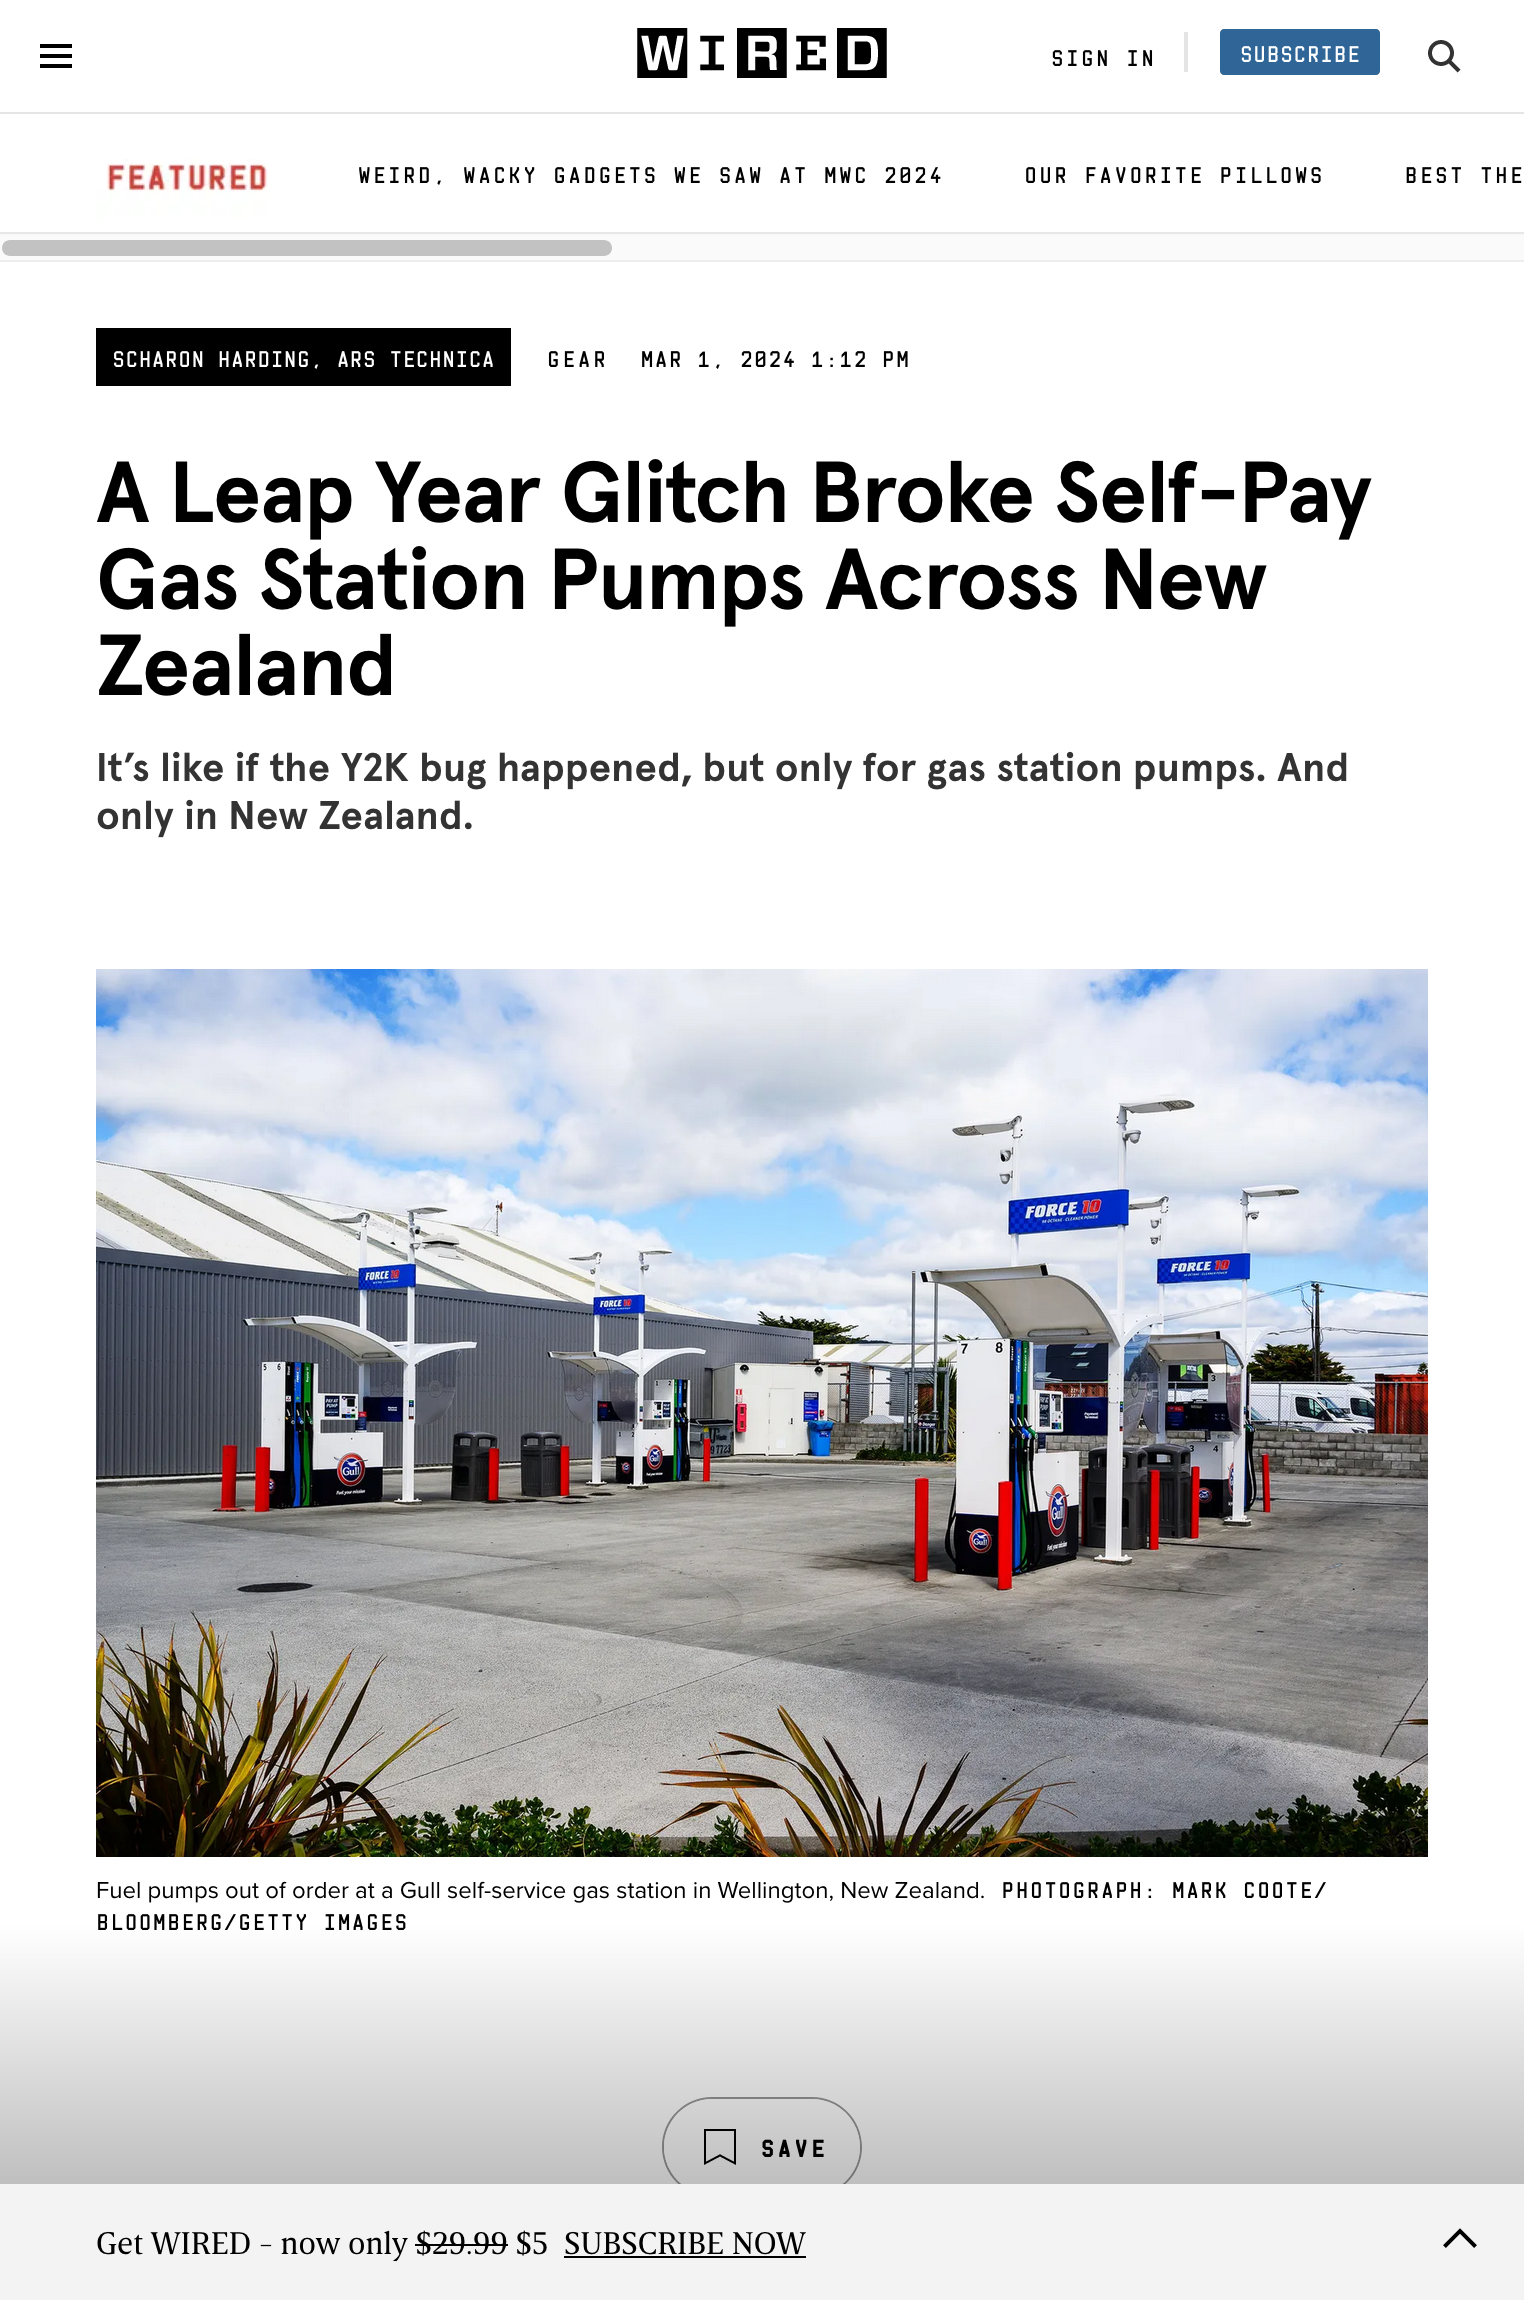
\includegraphics[width=0.3\linewidth]{images/bug.png}
    \caption{Screenshot of an article titled ``A Leap Year Glitch Broke Self-Pay Gas Station Pumps Across New Zealand''~\cite{ScharonHarding2024Mar}}
\end{figure}
\end{frame}

\begin{frame}{Software Testing in CS Education}
\begin{itemize}
    \item Integrating it into Computer Science curricula is challenging~\cite{garousi2020software, scatalon2020teaching}.
    \item Rational design paradigm is often used:
    \begin{itemize}
        \item Leading students to use a `developer approach' to testing~\cite{doorn2023towards}.
        \item Lacking empirical exploration and experimentation.
    \end{itemize} 
    \item We believe a shift to a design paradigm based on empiricism is needed.
    \item No knowledge on didactic approaches available, we think an approach based on abductive reasoning works.
    \item The use of serious games can be helpful.
    % \item We hypothesize that combining gamification with Socratic questioning can significantly improve the learning of software testing.
    % , fostering a shift towards an empirical design paradigm that emphasizes reflection-in-action and critical thinking.
    \item We started with the development of a serious game, where students devise a testing strategy for a system under test.
    % \item We use Socratic questioning as innovative approaches to enhance software testing education. 
    % These methods aim to foster engagement, practical application, immediate feedback, collaborative learning, and complex problem-solving.
\end{itemize}
\end{frame}

\section{Related Literature}

\begin{frame}[allowframebreaks]
    \frametitle{Theoretical background}
    \begin{itemize}
        \item Gamification is effective in software engineering education through: Real-world scenarios, Competitive elements, Immediate feedback, Interactive activities, and Collaboration~\cite{8658524}.
        \item Gamification is applicable across various educational strategies and contexts~\cite{informatics9040075, hirsh2022, Tan_Chong_2023}.%, enhancing engagement in software measurement processes, software testing education, and integration of modern technology stacks.
        \item Innovative tools and techniques include educational chatbots and the use of serious games in secure programming~\cite{10.1145/3350768.3352456,8802503}.
        % \item The educational impact and methodologies section discusses successful game-based interventions, methodologies for evaluating such interventions, and the Scrum Game Challenge for learning Scrum methodologies.
        \item Games should include meaningful competition and engagement, and there are risks of oversimplification and negative impacts like decreased intrinsic motivation~\cite{8658524}.
        \item Offline games such as TestSphere and `Would Heu-Risk It?'~\cite{BibEntry2023Sep} card games are used to enhance software testing discussions, collaboration, and strategy design.
        \item Interactive methods like `The TestOpsy'~\cite{ChrisKenst2022Jun} and `Blackbox Puzzles'~\cite{BibEntry2022Feb} focus on dissecting the testing process and improving problem-solving skills in software testing.
        % \item A systematic review on game-based learning's impact on argumentation skills emphasizes the importance of game elements, instructional supports, and learning theories for enhancing argumentation skills through game-based environments.
        \item Specific games such as `Testable'~\cite{8994972}, `Testing Maze'~\cite{10.1145/3613372.3614191}, `CleanGame'~\cite{10.1145/3350768.3352490}, and 'Code Defenders'~\cite{10.1145/3287324.3287471, 9155973} are designed to improve aspects of software testing education like unit testing, functional testing, code smell identification, and mutation testing.
    \end{itemize}
\end{frame}

\begin{frame}{Some existing games related to software testing}
\begin{figure}
    \centering
    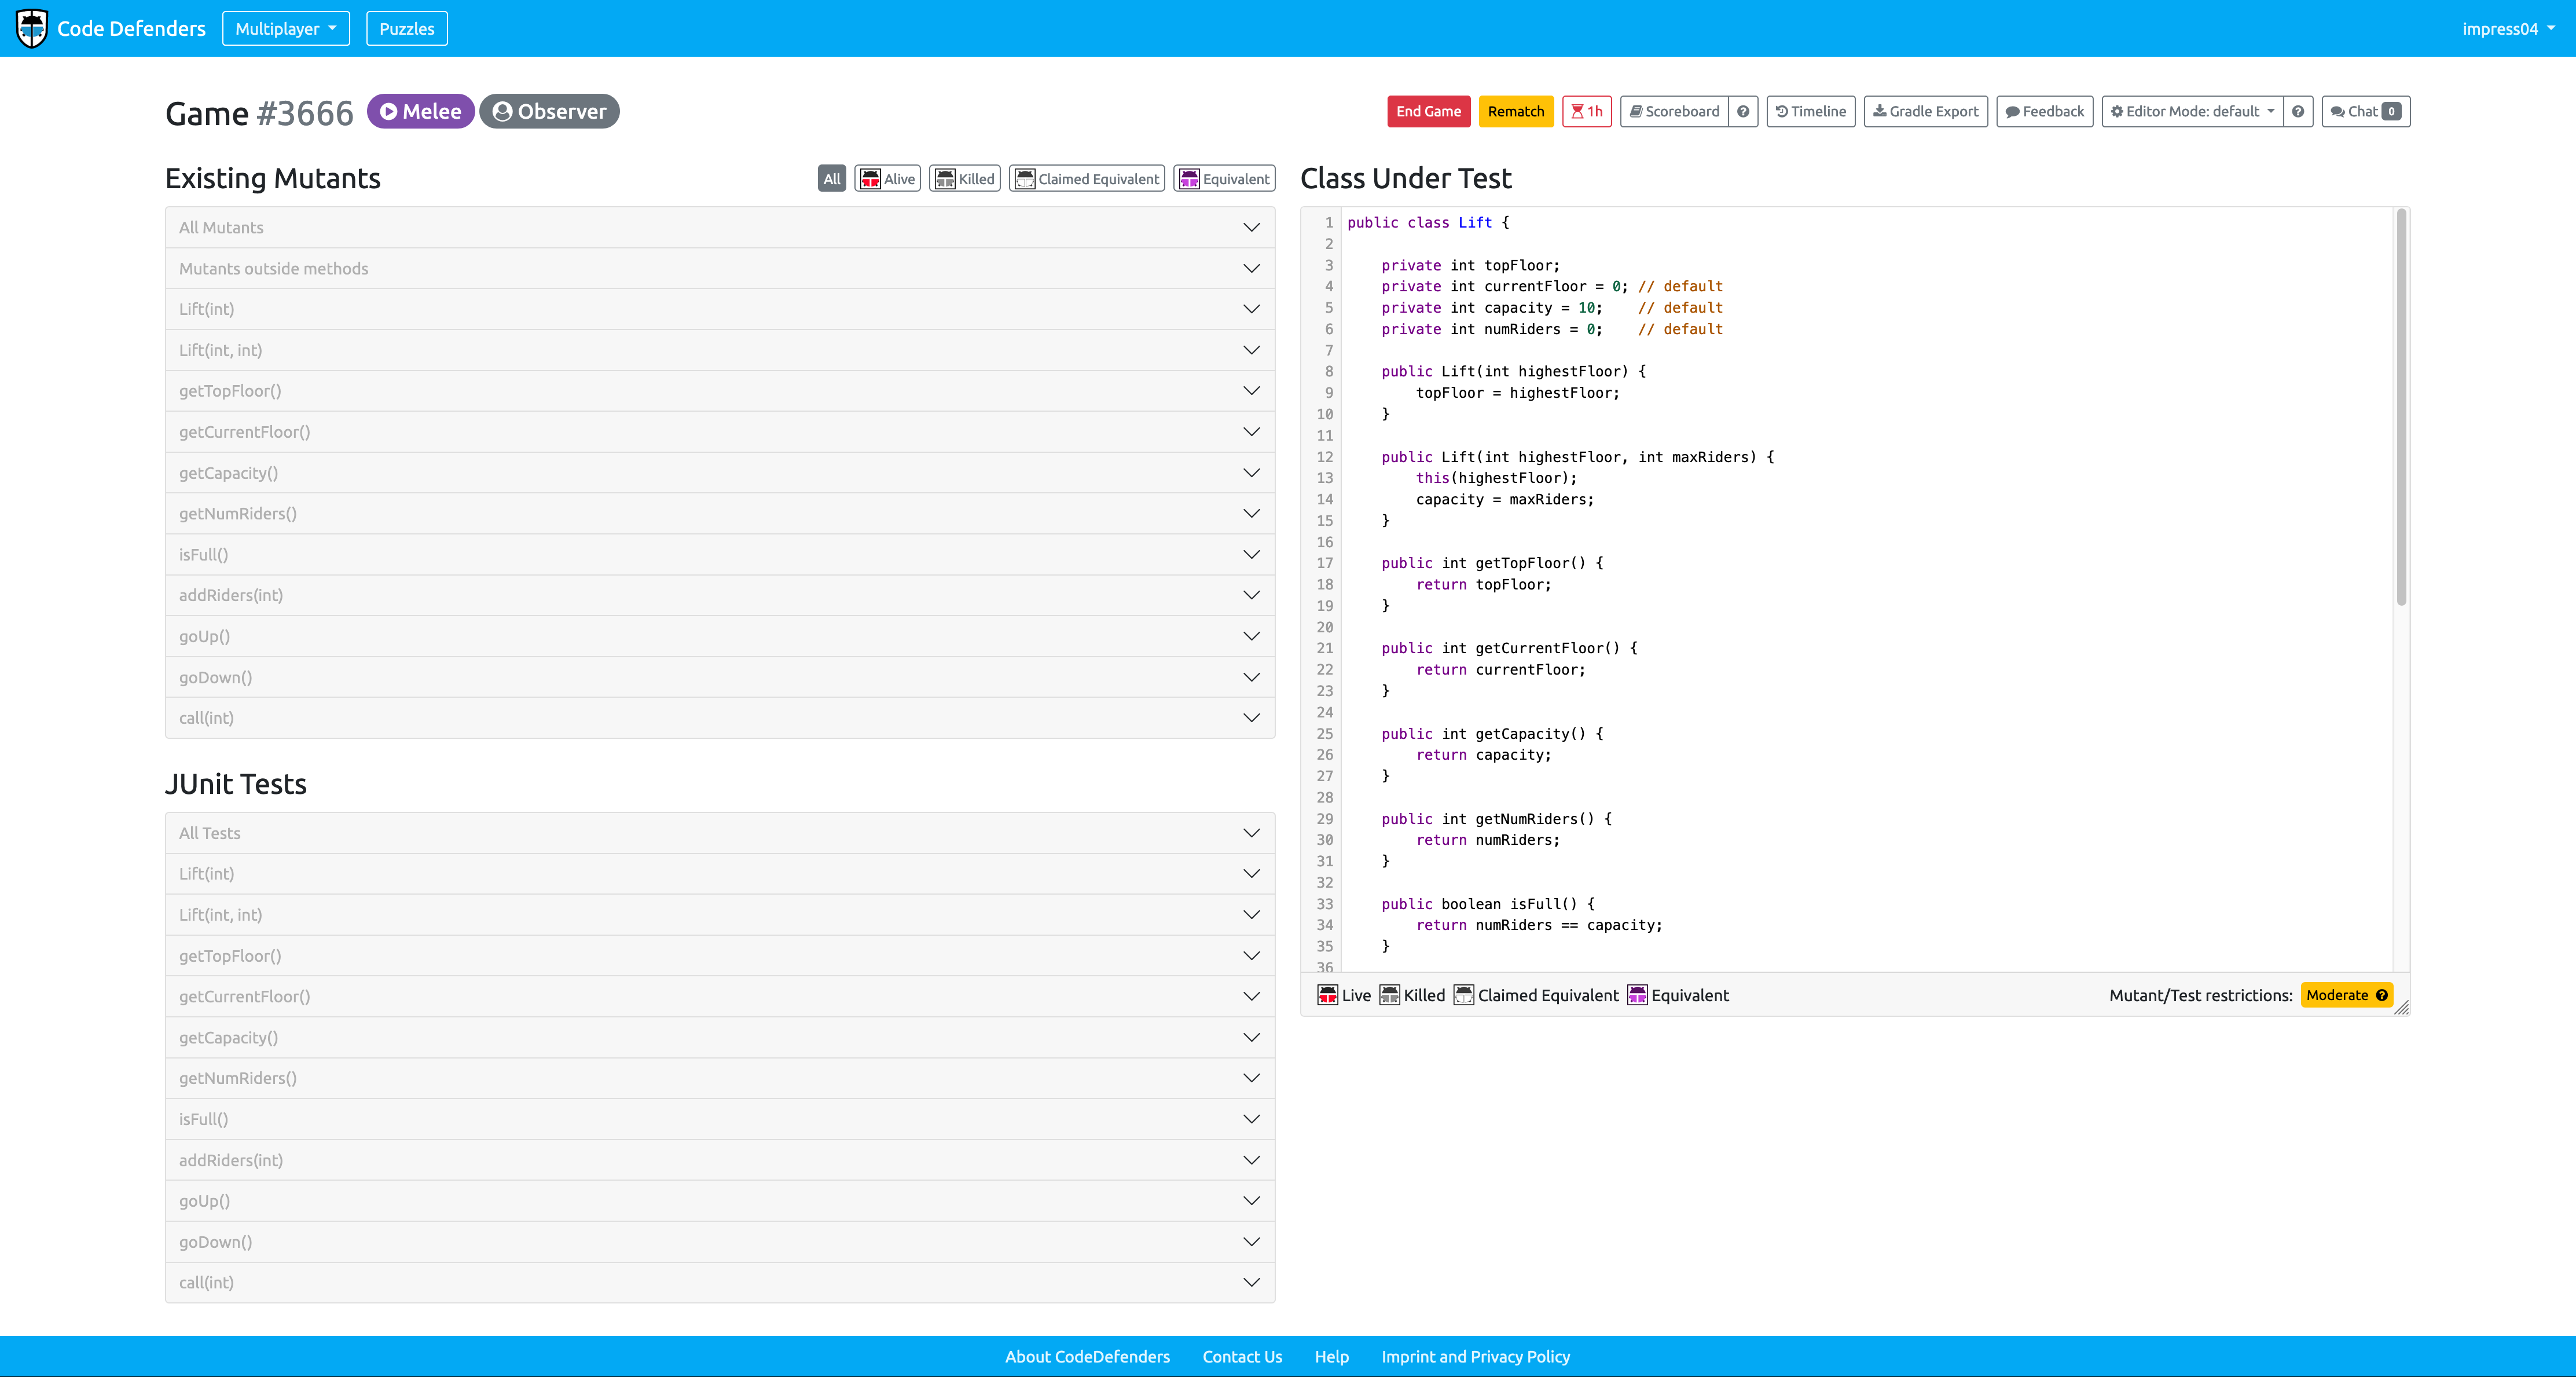
\includegraphics[width=0.75\linewidth]{images//games/codedefenders.png}
    \caption{CodeDefenders, an online game to learn mutation testing}
\end{figure}
\end{frame}

\begin{frame}{Some existing games related to software testing}
\begin{figure}
    \centering
    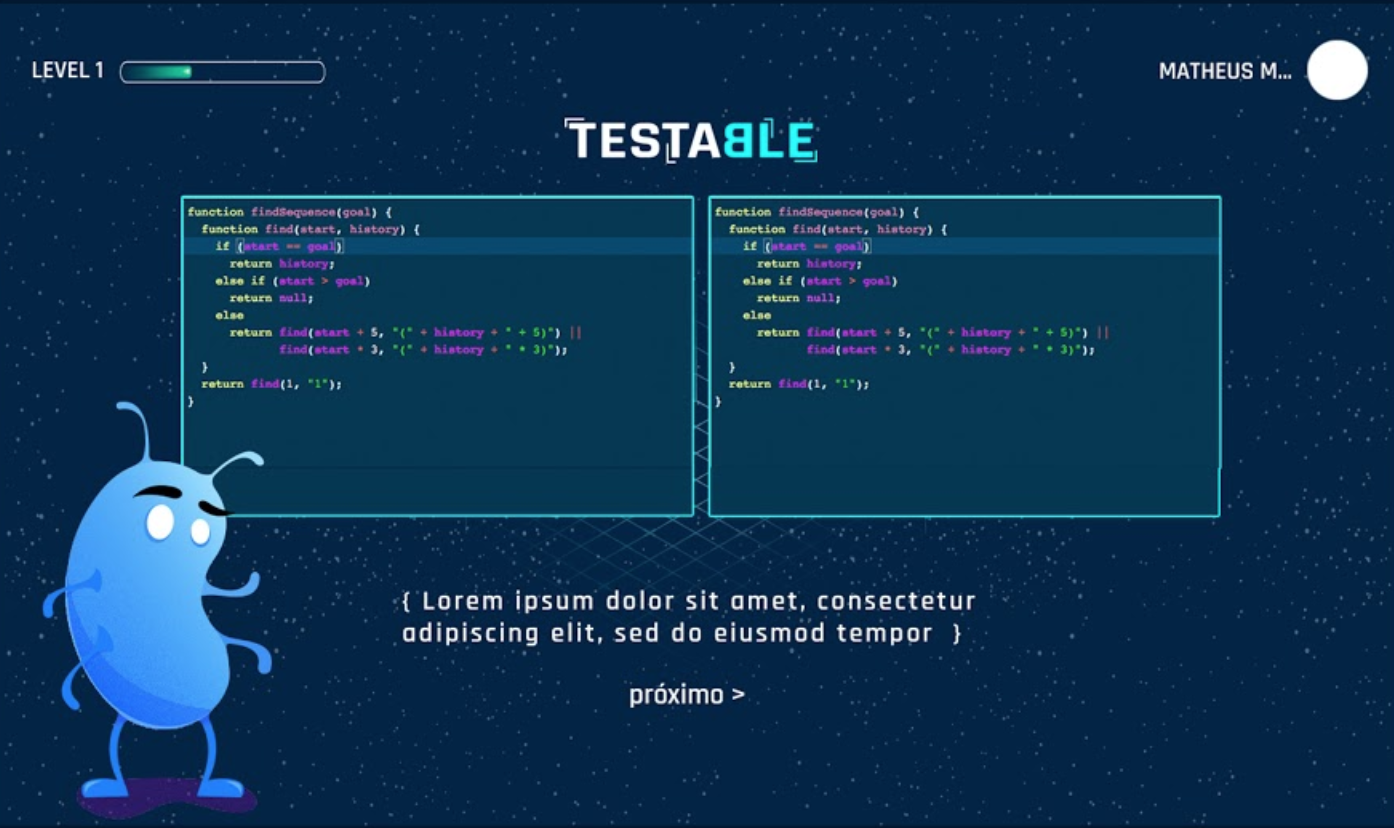
\includegraphics[width=0.75\linewidth]{images//games/testable}
    \caption{Testable - gamified tool to improve unit testing teaching}
\end{figure}
\end{frame}

\begin{frame}{Some existing games related to software testing}
\begin{figure}
    \centering
    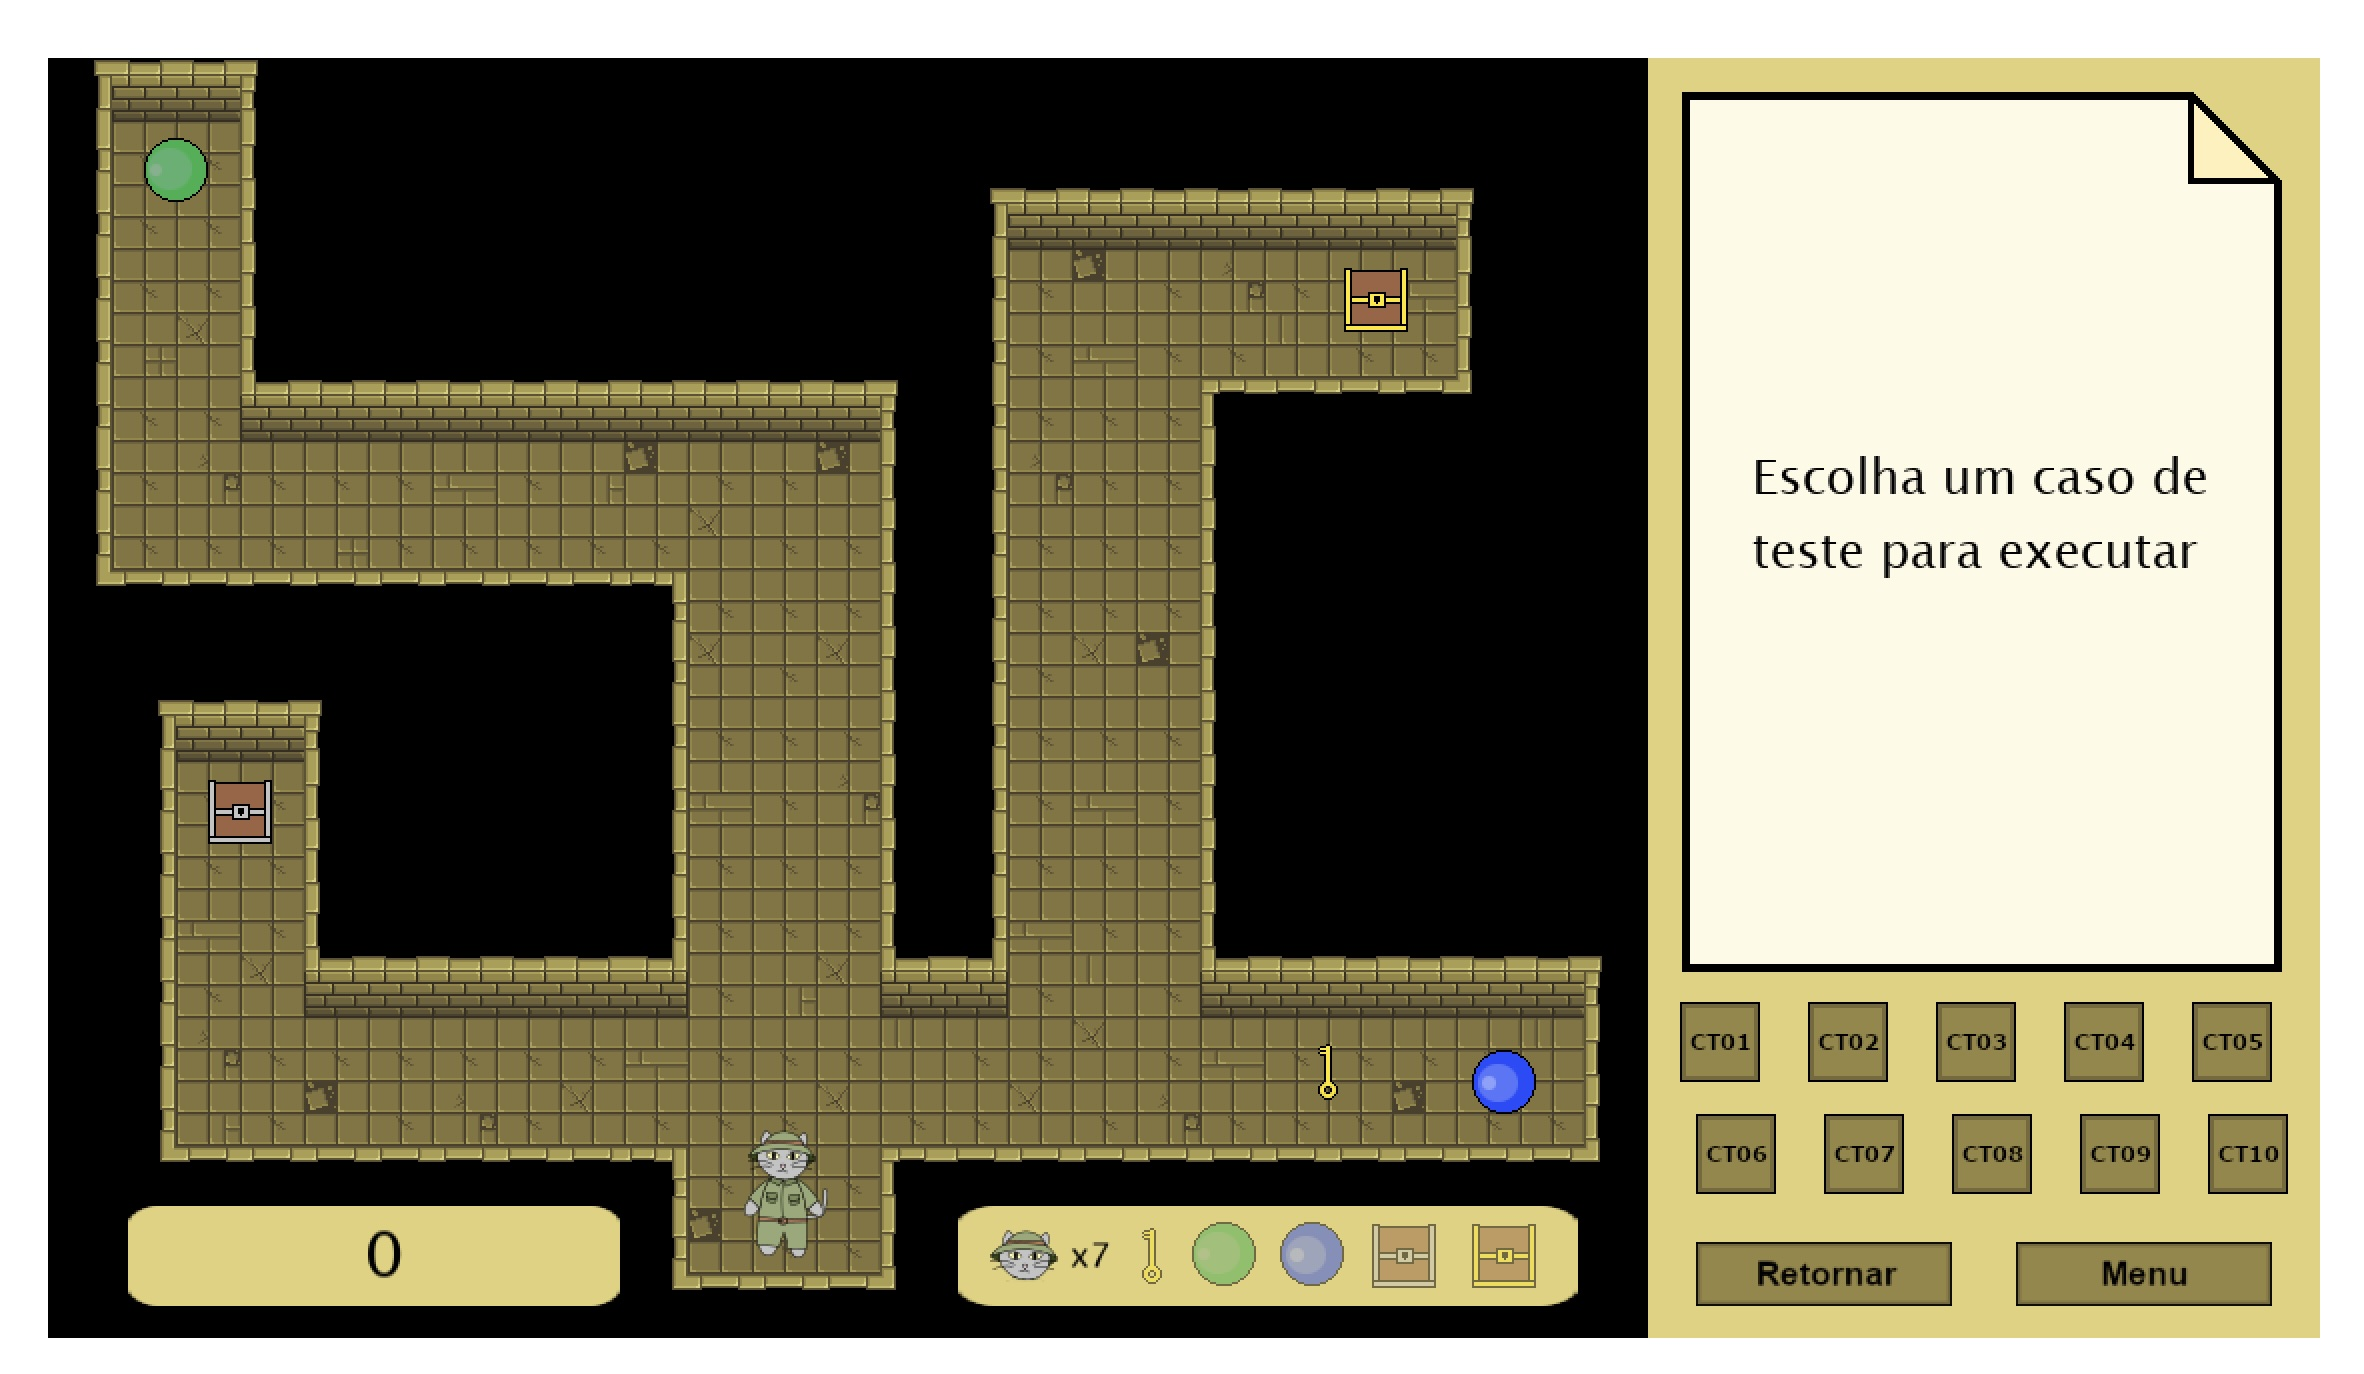
\includegraphics[width=0.75\linewidth]{images//games/testingmaze}
    \caption{Testing Maze, an educational puzzle game for teaching functional testing concepts and test specifications containing a fantasy narrative}
\end{figure}
\end{frame}

\begin{frame}{Some existing games related to software testing}
\begin{figure}
    \centering
    
\includegraphics[width=0.5\linewidth]{images//games/testsphere}
    \caption{The Card Deck That Gets You Thinking and Talking About Software Testing and Quality}
\end{figure}
\end{frame}

\begin{frame}{Some existing games related to software testing}
\begin{figure}
    \centering
    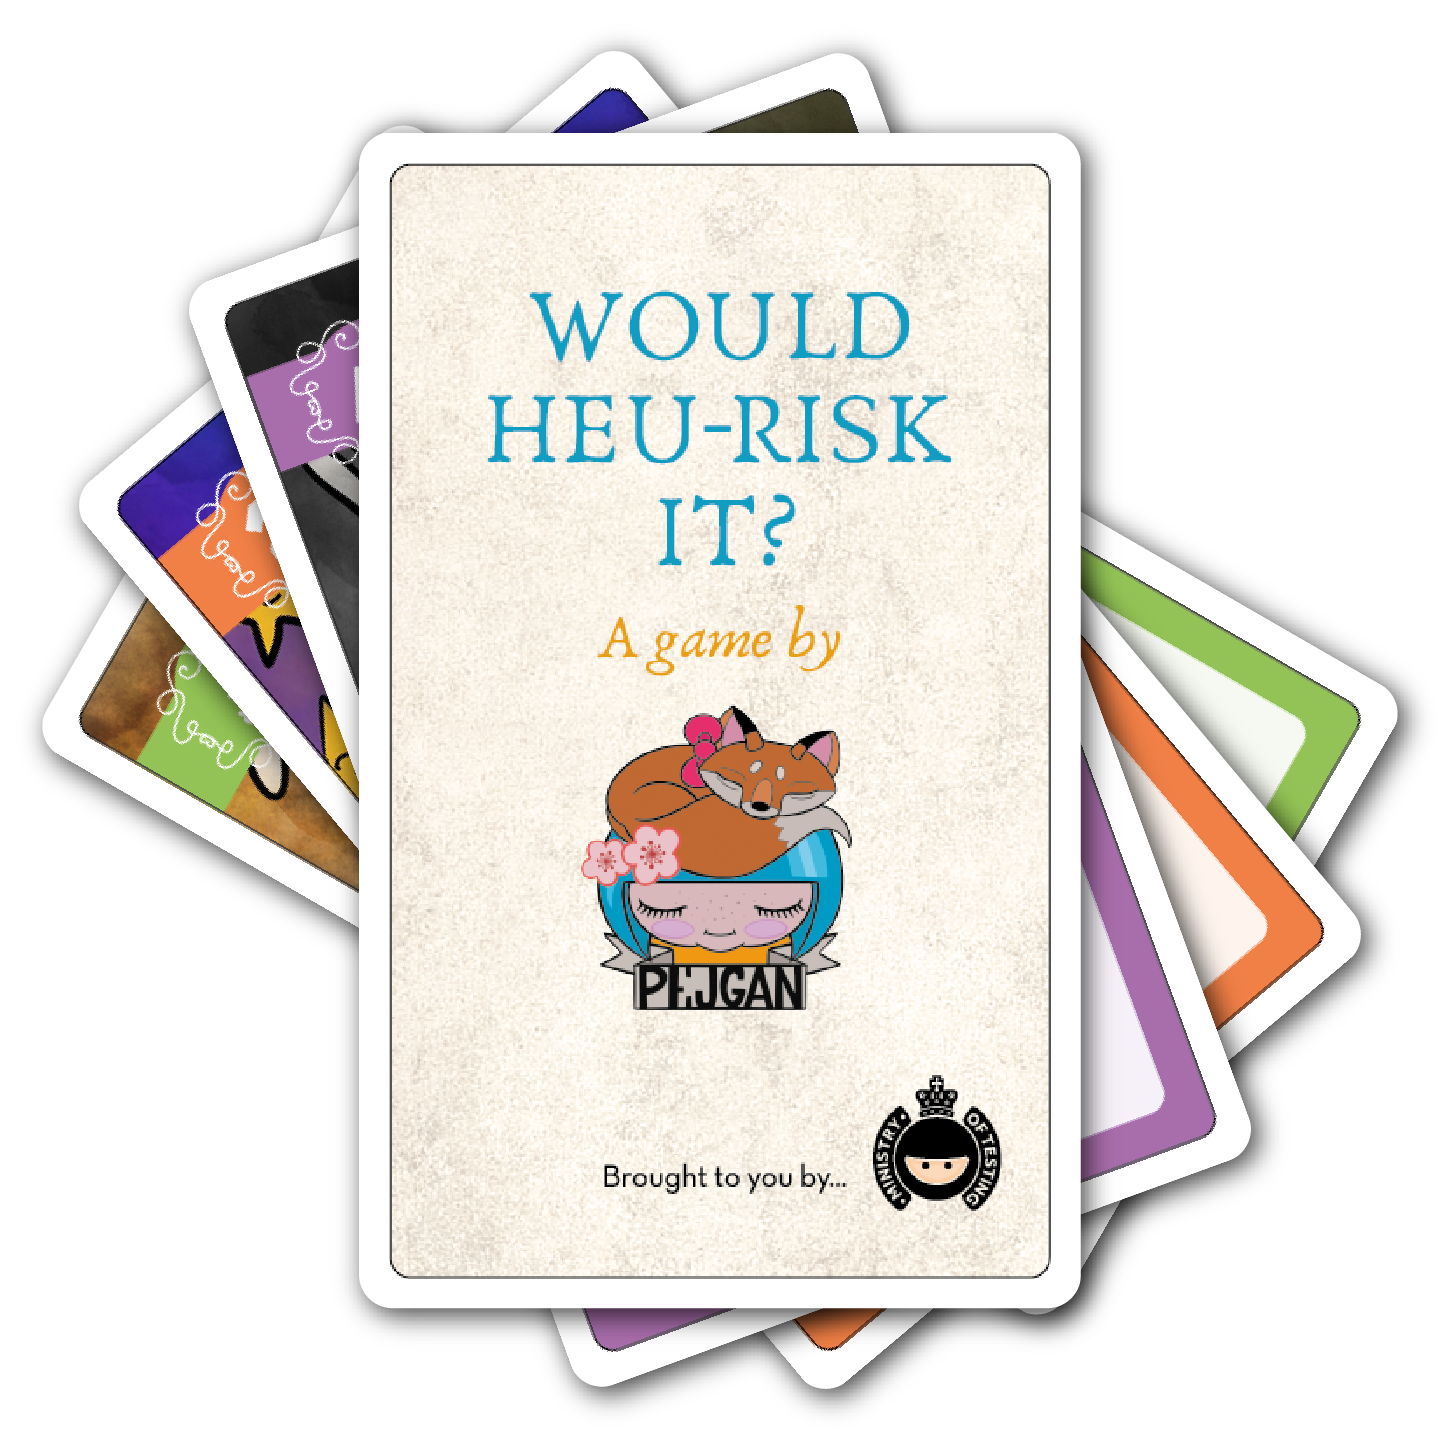
\includegraphics[width=0.5\linewidth]{images//games/would}
    \caption{`Would Heu-risk it?' is centered around risk analysis, heuristics, patterns/anti-patterns that affect us in designing, building, testing and running software}
\end{figure}
\end{frame}

\section{Problem of teaching software testing}

\begin{frame}{How we should teach software testing}
    \begin{itemize}
        \item Prevalence of 'developer approach' in testing by students.
        \item We need to shift their mental model.
        \item We need the right didactic approach.
    \end{itemize}
\end{frame}

\setbeamertemplate{background canvas}[ou plain]
\begin{frame}[noframenumbering,plain]
\begin{figure}
    \centering
    \vspace{-1cm}
    \hspace*{-1.2cm}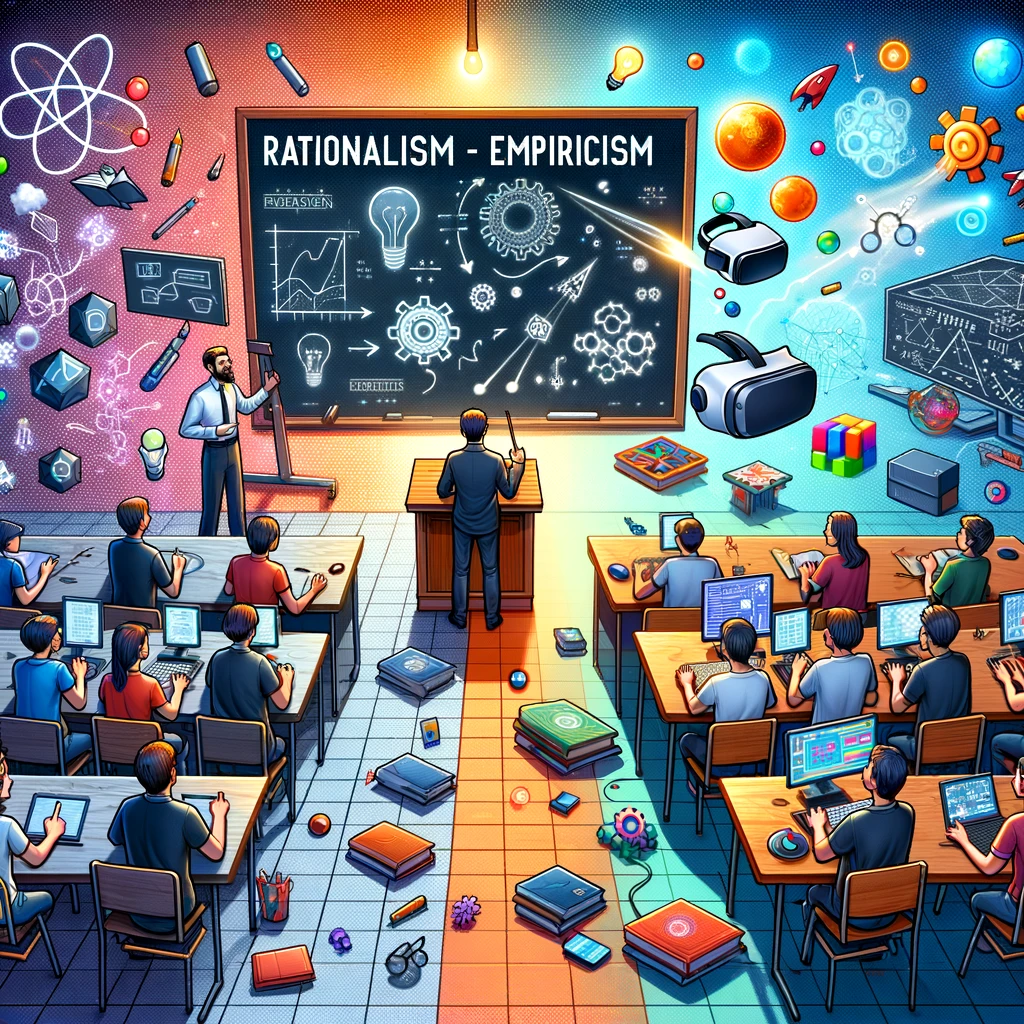
\includegraphics[width=1.2\linewidth]{images/plaatje.png}
\end{figure}
\end{frame}

\begin{frame}{Shift to Empiricism}
    \begin{itemize}
        \item Need for an empirical approach in teaching software testing.
        \item Emphasis on experimentation and heuristic-based learning.
        \item Students should follow an iterative process:
        \begin{itemize}
            \item form hypotheses based on observation and heuristics, 
            \item design tests, 
            \item execute them 
            \item and analyse the feedback.
        \end{itemize}
    \end{itemize}
\end{frame}

\begin{frame}{Didactics for software testing: \\Abductive Reasoning}
    \begin{blockquote}
    If it looks like a duck, and quacks like a duck, we have at least to consider the possibility that we have a small aquatic bird of the family Anatidae on our hands\\
    \textit{-- Douglas Adams}~\cite{adams1987dirk}.
    \end{blockquote}
\end{frame}

\begin{frame}{Abductive reasoning}
    Abductive reasoning is a form of logical inference that seeks the simplest and most likely conclusion from a set of observations.~\cite{ContributorstoWikimediaprojects2024Feb} 
    \begin{itemize}
        \item Basis for Design Thinking.
        \item Fits exploratory testing.
    \end{itemize}
\end{frame}

\section{Gamification}

\setbeamertemplate{background canvas}[ou plain]
\begin{frame}{Serious Game Development}
    \begin{itemize}
        \item Development process of a serious game for software testing.
        \item Incorporating empirical methods and critical thinking.
    \end{itemize}
\end{frame}

\begin{frame}{Pilot Study \& Results}
    \begin{itemize}
        \item Overview of the pilot study conducted.
        \item Improvements observed in students' testing strategies.
    \end{itemize}
    \textit{You work for a travel company. 
The sales department wants to know what the average age is of the people who booked their holidays with your company. One of the developers in your team has developed a program to calculate the average age for a hundred people at the time. The program can handle up to a hundred dates of births and calculates the average age in years. It gets its data from a remote server as a .txt file, where each line contains the name and the age.
}
\end{frame}

\begin{frame}{Wheel of socrative questions}
\begin{figure}
    \centering
    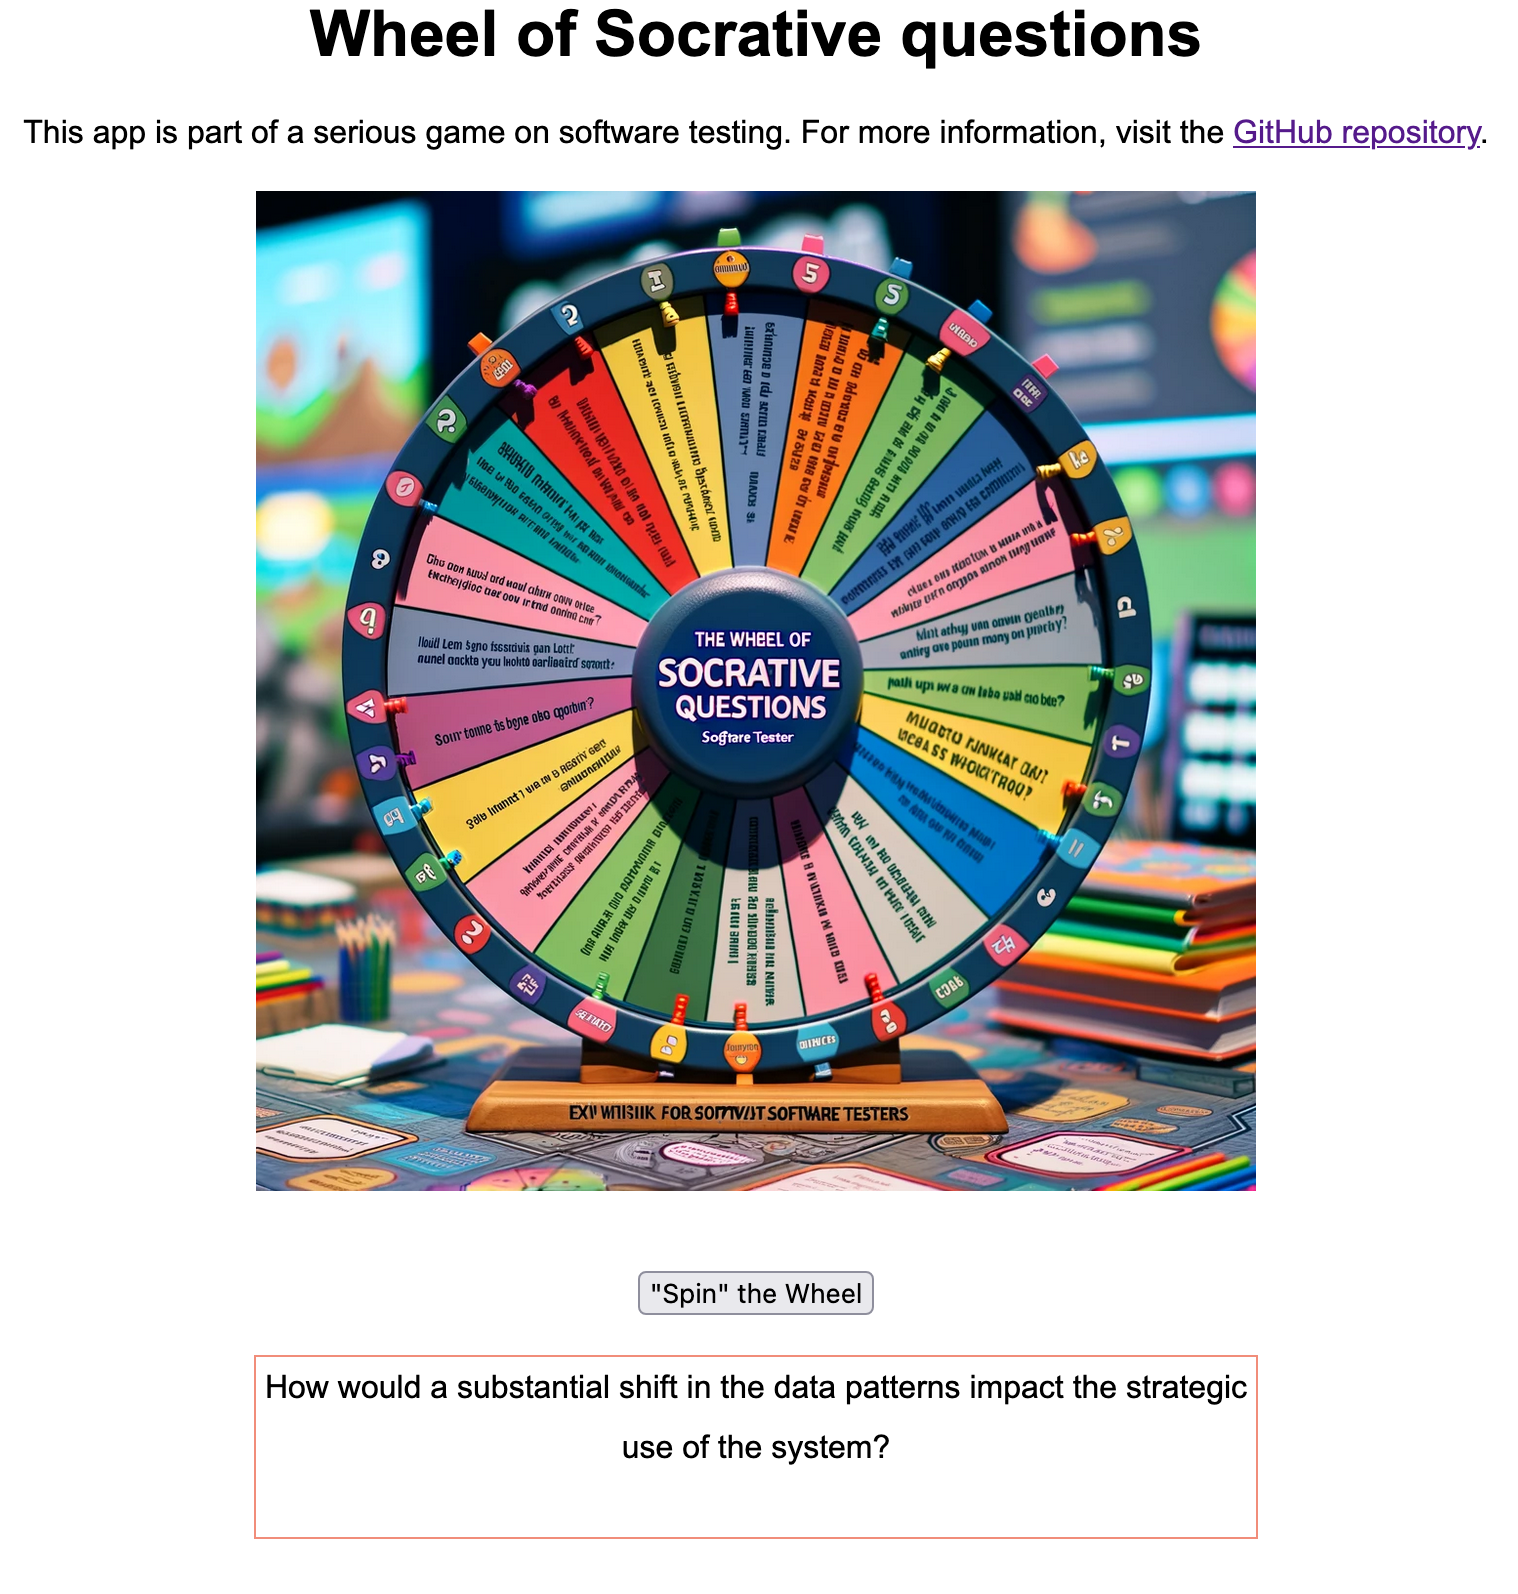
\includegraphics[width=0.5\linewidth]{images//wheel}
    \caption{"The Wheel of Socrative Questions," a game wheel designed for software testers}
\end{figure}
\end{frame}

% Socratic questions are a form of inquiry and discussion between individuals, based on asking and answering questions to stimulate critical thinking and to illuminate ideas. They are particularly useful in educational contexts, especially in subjects like computer science, where understanding concepts deeply is crucial. 

\section{Future work}

\setbeamertemplate{background canvas}[ou plain]
\begin{frame}{Future Work}
    \begin{itemize}
        \item Plans for further game development.
        \item Upcoming empirical studies in various educational contexts.
    \end{itemize}
\end{frame}

\section{Conclusion and thanks}

% \setbeamertemplate{background canvas}[ou birds]
% \begin{frame}{Conclusion}
%     \begin{itemize}
%         \item Summary of the shift towards an empirical approach.
%         \item Potential impact on software testing education.
%     \end{itemize}
% \end{frame}

\setbeamertemplate{background canvas}[ou plain]
\begin{frame}{Thanks for your attention}

% \begin{flushright}
% \vspace{2cm}
% \begin{minipage}{6cm}
\begin{itemize}
    \item Software Testing is important.
    \item A shift to an approach based on empirisism is needed.
    \item Gamification is an approach to support this in multiple educational contexts.
    \item We did a pilot to gain insights using socrative questioning.
    \item Game mechanics need to be added.
\end{itemize}

% \end{minipage}
% \end{flushright}

\begin{figure}
    \centering
    
\includegraphics[width=0.25\linewidth]{images//qr.png}
    \caption{More information about my research on \url{https://research.nielsdoorn.nl}}
\end{figure}
\end{frame}

\setbeamertemplate{background canvas}[ou plain]
\begin{frame}{Acknowledgements}
    This work was funded by the ENACTEST - European innovation alliance for testing education (ERASMUS+ Project number 101055874, 2022-2025).
\end{frame}

\setbeamertemplate{background canvas}[ou plain]
\begin{frame}[allowframebreaks]
    \frametitle{References}
    \printbibliography
\end{frame}

\end{document}
